\chapter{Policy Gradient Methods}
\label{ch:policygradientmethods}
Until now we have discussed so-called \textbf{action-value methods}, in which we learn the action values and use a policy (e.g., $\varepsilon$-greedy) to select actions based on those estimates. A possible alternative would be to have a different set of methods that could learn a \textbf{parametrized policy that allowed them to select actions without consulting a value function} (a value function might be used to learn the policy parameter, but it is not required for action selection; we will keep using the $\boldsymbol{w} \in \mathbb{R}^d$ notation for the weight vector of the value function).

For \textbf{policy networks} we will use $\boldsymbol{\theta}$ to indicate the \textbf{policy’s parameter vector}, with $\boldsymbol{\theta} \in \mathbb{R}^{d'}$. The probability of taking an action $a$ at time $t$, given that the environment is in state $s$ at time $t$ with parameter $\boldsymbol{\theta}$, will then be:

\begin{equation*}
    \pi \left( a \middle\vert s, \boldsymbol{\theta} \right) = \text{Pr}\left\{ A_t = a \ \middle\vert \ S_t = s, \boldsymbol{\theta}_t = \boldsymbol{\theta} \right\}
\end{equation*}

The methods that will be introduced in this chapter will learn the policy parameter $\boldsymbol{\theta}$ by means of (the gradient of) a scalar performance measure $J(\boldsymbol{\theta})$. Since these methods will seek to \textit{maximize} performance\footnote{Earlier we were trying to \textbf{minimize the error} in the Q-value estimation, whereas now we are trying to \textbf{maximize the performance} of our policy.}, their updates will work towards approximating \textbf{gradient ascent} in $J$:

\begin{equation}
    \boldsymbol{\theta}_{t+1} = \boldsymbol{\theta}_t + \alpha \widehat{\nabla J(\boldsymbol{\theta}_t)}
    \label{eq:ch8-gradientascentupdate}
\end{equation}

Where $\widehat{\nabla J(\boldsymbol{\theta}_t)} \in \mathbb{R}^{d'}$ is a stochastic estimate whose expectation approximates the gradient of the performance measure with respect to its argument $\boldsymbol{\theta}_t$. In simpler terms, we perform our weight correction in the direction that, based on our estimate of $J(\boldsymbol{\theta})$, will lead to a gradient ascent. Methods that follow this schema are called \textbf{policy gradient methods}.

\section{Policy approximation and its advantages}
In policy gradient methods, the policy can be parametrized in any way, with one caveat: $\pi \left( a \middle\vert s, \boldsymbol{\theta} \right)$ must be differentiable with respect to its parameters, that is, as long as $\nabla \pi \left( a \middle\vert s, \boldsymbol{\theta} \right)$ exists and is finite $\forall s \in \mathcal{S}, a \in \mathcal{A}(s)$ and $\boldsymbol{\theta} \in \mathbb{R}^{d'}$. In practice, however, to ensure exploration it is usually required that the policy never becomes deterministic.

A common way to parametrize policies is to form a \textbf{parametrized numerical preference} $h(s,a,\boldsymbol{\theta}) \in \mathbb{R}$ for each state-action pair (this is often the case when the action space is discrete and not too large). The actions with the highest preferences in each state will then be given the highest probabilities of being selected, typically according to an exponential soft-max distribution as such:

\begin{equation}
    \pi \left(a \middle\vert s, \boldsymbol{\theta} \right) \doteq \frac{e^{h(s,a,\boldsymbol{\theta})}}{\sum_{b} h(s,b,\boldsymbol{\theta})}
    \label{eq:ch8-softmaxinactionpreferencesparametrization}
\end{equation}

Where $e \approx 2.71828$ is Euler’s number, the base of the natural logarithm. This type of policy parametrization is called \textbf{soft-max in action preferences}.

The parametrization of the action preferences is arbitrary, too. The $h(s,a,\boldsymbol{\theta}) \in \mathbb{R}$ values might be computed, for example, by a deep artificial neural network, where $\boldsymbol{\theta}$ is the vector of all the connection weights of the network (like in the case of AlphaGo). This is just one of the options, but it helps us scale up.

One advantage of parametrizing policies according to the \textit{soft-max in action preferences} is that the approximate policy can approach a deterministic one, whereas with $\varepsilon$-greedy we would always have an $\varepsilon$ probability of selecting a random action. We could also select actions according to a soft-max distribution based on action values, but this alone would not allow the policy to approach a deterministic one. The action-value estimates would end up converging to their true values, which would differ by a finite amount, causing the soft-max function to output specific probabilities, and not just 0 and 1. Action preferences are different because they \textit{do not approach specific values}; instead, \textit{they are driven to produce the optimal stochastic policy}: if the optimal policy is deterministic, then the preferences of the optimal actions will be driven infinitely higher than all suboptimal actions (if permitted by the parametrization).

A second advantage is that this method enables the selection of actions with arbitrary probabilities. This means that, when dealing with problems where the best approximate policy is stochastic (such as in rock-paper-scissors), we can even learn to choose one of the available actions with equal probability, something that is not possible with action-value methods.

Last, and perhaps the simplest, advantage that policy parametrization may have over action-value parametrization is that the policy may be a simpler function to approximate, converging faster and more smoothly.

\section{Policy Gradient Theorem}
As we just said, with continuous policy parametrization the action probabilities change smoothly as a function of the learned parameter, whereas in $\varepsilon$-greedy selection the action probabilities may change dramatically for an arbitrary small change in the estimated action values, if that change results in a different action having the maximal value. Largely because of this, policy gradient methods have stronger convergence guarantees compared to action-value methods.

Let us consider \textbf{episodic learning}, for which we define the performance measure as the value of the start state of the episode\footnote{Our objective is to play to the best of our abilities, which means maximizing the expected cumulative rewards $G$. We obtain exactly that by maximizing the value of the initial state.}. We simplify the notation (without losing any meaningful generality) by assuming that every episode starts in some particular (non-random) state $s_0$. The performance is then defined as:

\begin{equation*}
    J(\boldsymbol{\theta}) \doteq v_{\pi_{\boldsymbol{\theta}}}(s_0)
\end{equation*}

Where $v_{\pi_{\boldsymbol{\theta}}}$ is the true value function for $\pi_{\boldsymbol{\theta}}$, the policy determined by $\boldsymbol{\theta}$. The issue now becomes how to change the policy parameter $\boldsymbol{\theta}$ by means of function approximation in a way that ensures improvement.

Doing so is more complicated than it may seem from a superficial look. Performance --as in, how good our policy is-- depends on two things:

\begin{itemize}
    \item The actions we choose in a certain state.
    \item The states that the policy makes us go through.
\end{itemize}

Both factors are affected by the policy parameter. However, while it is easy to compute, given a state and knowledge of the parametrization, the effect of the policy parameter on the actions, the effect of the policy on the state distribution (the states that we end up visiting) is a function of the environment, which is typically unknown, making it impossible to estimate. 

How can we then perform gradient ascent (formula \ref{eq:ch8-gradientascentupdate}) if the gradient of the performance with respect to the policy parameter depends on the unknown effect of policy changes on the state distribution?  The \textbf{policy gradient theorem} comes to our rescue, providing us with an analytic expression of the gradient that does not involve the derivative of the state distribution, as we can see below:

\begin{equation}
    \nabla J(\boldsymbol{\theta}) \propto \sum_s \mu(s) \sum_a q_\pi(s,a) \nabla\pi(a \vert s, \boldsymbol{\theta})
    \label{eq:ch8-policygradienttheorem}
\end{equation}

Where the gradients are column vectors of partial derivatives with respect to the components of $\boldsymbol{\theta}$ and $\pi$ denotes the policy corresponding to parameter vector $\boldsymbol{\theta}$. $\mu(s)$ is the \textbf{on-policy distribution} under policy $\pi$ and it describes the normalized frequency with which states are encountered while the agent is selecting actions according to $\pi$ or, to put it differently, it is the normalized fraction of time spent in each state. A proof for this formula can be found in Sutton and Barto’s book on page 325.

We might then ask: the policy gradient theorem only provides us with something that is \textit{proportionate to} the gradient, and not \textit{equal to}, does it still work? The answer is yes, in the weight update formula, in fact, we can use the step size $\alpha$ to turn this proportionality into an equality by setting it to the average length of an episode.

\section{REINFORCE: Monte Carlo Policy Gradient}
As we mentioned in the beginning of this chapter, our strategy of stochastic gradient ascent is based on $\widehat{\nabla J(\boldsymbol{\theta}_t)}$, a stochastic estimate whose expectation approximates the gradient of the performance measure with respect to its argument $\boldsymbol{\theta}_t$. Thanks to the policy gradient theorem, this approximation is sufficient, and we can ``absorb'' the error of this estimate in the step size constant $\alpha$. 

The problem at hand now becomes finding a way of sampling whose expectation equals or approximates the expression given by the policy gradient theorem\footnote{Since the update formula is based on $\widehat{\nabla J(\boldsymbol{\theta}_t)}$, a stochastic estimate of the gradient of the performance function with respect to its parameters, we need to find a way to sample $\nabla J(\boldsymbol{\theta})$. We do so by applying the policy gradient theorem.}. Given the definition of $\mu$ we gave earlier, we can see the right-hand side of the theorem as a sum over states weighted by how often the state occurs under the target policy $\pi$. If $\pi$ is followed, then the states will be encountered in these proportions, which means that:

\begin{equation}
    \begin{split}
        \nabla J(\boldsymbol{\theta}) &\propto \sum_s \mu(s) \sum_a q_\pi(s,a) \nabla\pi(a \vert s, \boldsymbol{\theta}) \\
        &= \mathbb{E}_\pi \Bigg[ \sum_a q_\pi (S_t, a) \nabla \pi (a \vert S_t, \boldsymbol{\theta}) \Bigg]
    \end{split}
    \label{eq:ch8-statesampledpolicygradient}
\end{equation}

As a reminder, we defined $\mathbb{E}_\pi \left[\cdot\right]$ as the expected value of a random variable given that the agent follows $\pi$.

In theory, we could stop here and instantiate the stochastic gradient-ascent algorithm (\ref{eq:ch8-gradientascentupdate}) as:

\begin{equation*}
    \boldsymbol{\theta}_{t+1} \doteq \boldsymbol{\theta}_{t} + \alpha \sum_a \hat{q}(S_t,a,\boldsymbol{w}) \nabla \pi (a \vert S_t, \boldsymbol{\theta})
\end{equation*}

Where $\hat{q}$ is some learned approximation of $q_\pi$. We obtained an \textbf{all-action method}, because its update involves all the actions in each update, but our focus is on REINFORCE, whose update at time $t$ involves just $A_t$, the action actually taken at time $t$.

We continue our derivation of REINFORCE by introducing $A_t$ in the same way we introduced $S_t$ just now: by replacing a sum over the random variable’s possible values by an expectation under $\pi$ and then sampling the expectation. Equation \ref{eq:ch8-statesampledpolicygradient} now becomes:

\begin{equation}
    \begin{split}
        \nabla J(\boldsymbol{\theta}) &\propto \mathbb{E}_\pi \Bigg[ \sum_a q_\pi (S_t, a) \nabla \pi (a \vert S_t, \boldsymbol{\theta}) \Bigg] \\
        &= \mathbb{E}_\pi \Bigg[ \sum_a \pi (a \vert S_t, \boldsymbol{\theta}) \cdot q_\pi (S_t, a) \nabla \pi (a \vert S_t, \boldsymbol{\theta}) \cdot \frac{1}{\pi (a \vert S_t, \boldsymbol{\theta})} \Bigg] \\
        &= \mathbb{E}_\pi \Bigg[ \mathbb{E}_\pi \left[ q_\pi (S_t, A_t) \right] \frac{\nabla \pi (a \vert S_t, \boldsymbol{\theta})}{\pi (a \vert S_t, \boldsymbol{\theta})} \Bigg] \quad \text{since } \mathbb{E}_\pi \left[\mathbb{E}_\pi[\cdot]\right] = \mathbb{E}_\pi [\cdot] \\
        &= \mathbb{E}_\pi \Bigg[ q_\pi (S_t, A_t) \frac{\nabla \pi (a \vert S_t, \boldsymbol{\theta})}{\pi (a \vert S_t, \boldsymbol{\theta})} \Bigg] \quad \text{since } \mathbb{E}_\pi \left[G_t \vert S_t, A_t \right] = q_\pi (S_t, A_t) \\
        &= \mathbb{E}_\pi \Bigg[ G_t \frac{\nabla \pi (a \vert S_t, \boldsymbol{\theta})}{\pi (a \vert S_t, \boldsymbol{\theta})} \Bigg]
    \end{split}
    \label{eq:ch8-stateandactionsampledpolicygradient}
\end{equation}

We now have an expression that can be sampled on each time step and whose expectation is proportional to the gradient. Using this sample to instantiate our generic stochastic gradient ascent algorithm, we obtain the REINFORCE update rule:

\begin{equation}
    \boldsymbol{\theta}_{t+1} \doteq \boldsymbol{\theta}_{t} + \alpha G_t \frac{\nabla \pi (a \vert S_t, \boldsymbol{\theta})}{\pi (a \vert S_t, \boldsymbol{\theta})}
    \label{eq:ch8-reinforceupdaterule}
\end{equation}

With this rule, each increment is proportional to the product of a return $G_t$ and a vector, the gradient of the probability of taking the action actually taken divided by the probability of taking that action. The vector is the direction in the parameter space that most increases the probability of repeating the action $A_t$ on future visits to state $S_t$. The update increases the parameter vector in this direction proportional to the return, and inversely proportional to the action probability. The former makes sense because it causes the parameter to move most in the directions that favor actions that yield the highest return. The latter makes sense because otherwise actions that are selected frequently are at an advantage (the updates will be more often in their direction) and might win out even if they do not yield the highest return.

If we then apply the identity $\nabla \ln{x} = \frac{\nabla x}{x}$, we obtain the final formulas:

\begin{equation}
    \nabla J(\boldsymbol{\theta}) \propto \mathbb{E}_\pi \Big[ G_t \nabla \ln{\pi (a \vert S_t, \boldsymbol{\theta})} \Big]
    \label{eq:ch8-finalreinforcepolicygradient}
\end{equation}

\begin{equation}
    \boldsymbol{\theta}_{t+1} \doteq \boldsymbol{\theta}_{t} + \alpha G_t \nabla \ln{\pi (a \vert S_t, \boldsymbol{\theta})}
    \label{eq:ch8-finalreinforceupdaterule}
\end{equation}

A pseudocode implementation of REINFORCE is provided here:

\begin{algorithm}[H]
\DontPrintSemicolon
\SetAlgoVlined
\KwIn{a differentiable policy parametrization $\pi (a \vert S_t, \boldsymbol{\theta})$}
\Parameters{step size $\alpha > 0$}
\Initialize{policy parameter $\boldsymbol{\theta} \in \mathbb{R}^{d'}$ (e.g., to $\boldsymbol{0}$)}

 \Loop{for each episode}{
    Generate an episode $S_0, A_0, R_1, ..., S_{T-1}, A_{T-1}, R_T$, following $\pi(\cdot \vert \cdot, \boldsymbol{\theta})$\;
    \Loop{for each step of the episode $t = 0, 1, ..., T-1$}{
        $G \leftarrow \sum_{k = t+1}^{T} R_k$\;
        $\boldsymbol{\theta} \leftarrow \boldsymbol{\theta} + \alpha G \nabla \ln{\pi (A_t \vert S_t, \boldsymbol{\theta})}$
    }
 }
\caption{REINFORCE: Monte-Carlo Policy-Gradient Control (episodic) for $\pi_*$}
\end{algorithm}

To have a better idea of how this is could be put into practice in a neural network, we can look at figure \ref{fig:ch8-reinforcepolicynetwork}.

\begin{figure}[hbp]
    \centering
    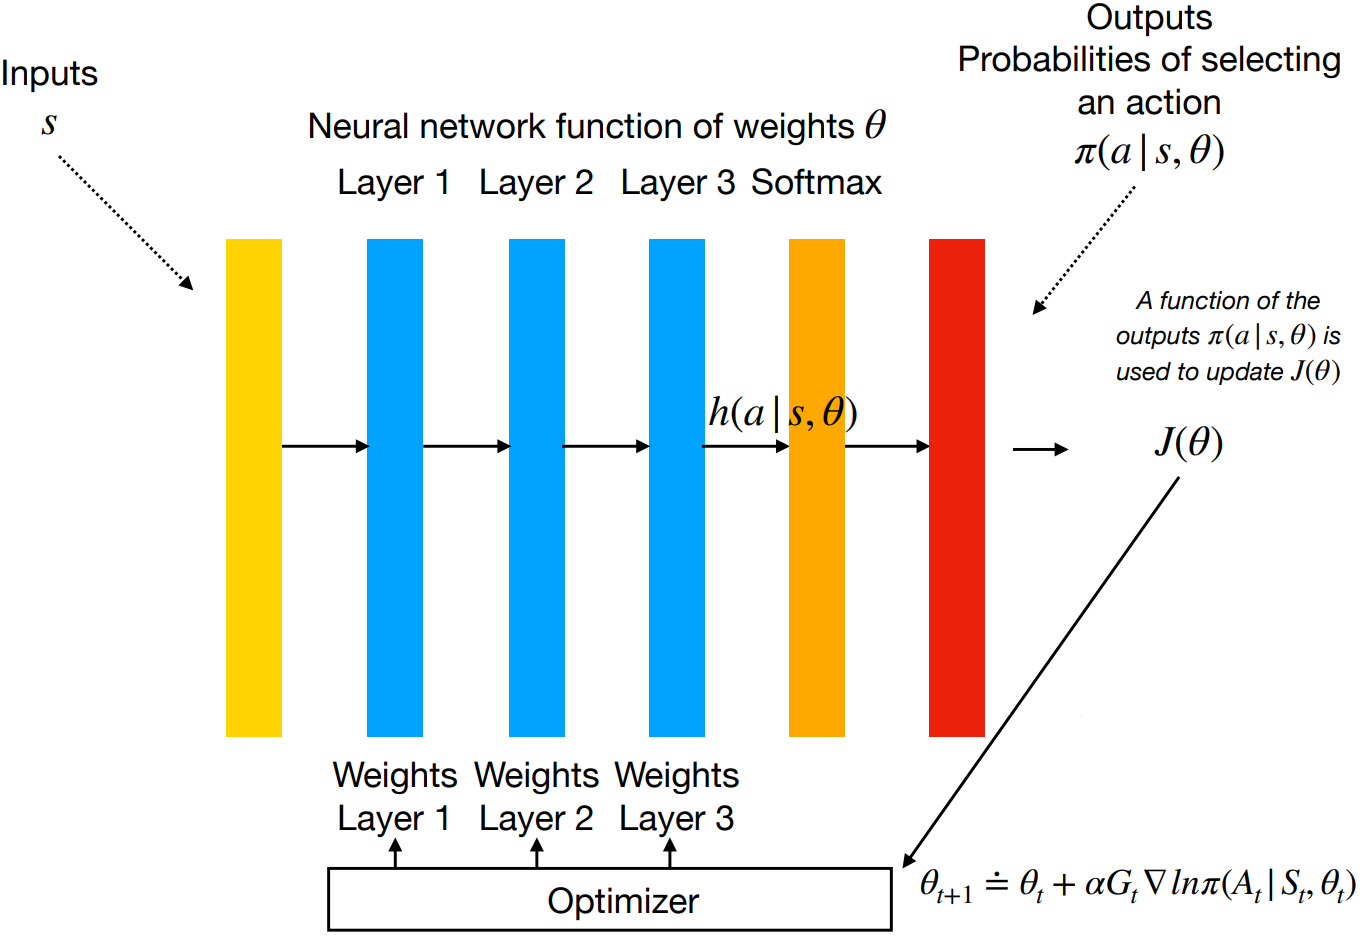
\includegraphics[scale=0.35]{Images/Chapter 8/reinforce-policy-network.png}
    \caption{A neural network using REINFORCE}
    \source{Prof. Mirco Musolesi}
    \label{fig:ch8-reinforcepolicynetwork}
\end{figure}

\subsection{Stochastic Gradient Ascent}
What we have seen in picture \ref{fig:ch8-reinforcepolicynetwork} works, except for one not-so-minor detail: neural networks (and the backpropagation algorithm) work by minimizing the loss function, performing stochastic gradient \textit{descent}, which is the opposite of what we want to do (an explanation of how stochastic gradient descent works can be found in \autoref{subsection:gradient-based-optimization}).

A simple --but effective-- trick to have neural networks perform stochastic gradient \textit{ascent} is then to have a new function $J' (\boldsymbol{\theta})$ that is the opposite of $J(\boldsymbol{\theta})$. Formally, we will have:

\begin{itemize}
    \item $J' (\boldsymbol{\theta}) = -(G_t \ln{\pi} - 0) = -G_t \ln{\pi}$
    \item $\nabla J' (\boldsymbol{\theta}) = -G_t \nabla \ln{\pi}$
\end{itemize}

\subsection{How well does REINFORCE perform?}
As a stochastic gradient method, REINFORCE has good theoretical convergence properties: by construction, the expected update over an episode is in the same direction as the performance gradient. This assures an improvement in expected performance for sufficiently small $\alpha$, and convergence to a local optimum under standard stochastic approximation conditions for decreasing $\alpha$. However, being a Monte Carlo method, REINFORCE suffers from high variance\footnote{The variance is high because the return $G_t$ is the sum of many random variables $R_t, R_{t+1},...,R_T$, each of which depends on distributions not just in the case of the reward $R$ received by the environment, but also in the choice of action $A$, and the state transition dynamics that pick each $S$. Ref: \url{https://stats.stackexchange.com/questions/364997/what-is-intuition-behind-high-variance-of-monte-carlo-method}}, causing a slow learning process. To deal with this problem, we can use \textbf{baselines} or \textbf{actor-critic} methods.

\section{REINFORCE with Baseline}
To overcome the issue of high variance in Monte Carlo updates, we can generalize the \textit{policy gradient theorem} (equation \ref{eq:ch8-policygradienttheorem}) by including a comparison of the action value to an arbitrary \textbf{baseline} $b(s)$:

\begin{equation}
    \nabla J(\boldsymbol{\theta}) \propto \sum_s \mu(s) \sum_a \big(q_\pi(s,a) - b(s) \big) \nabla\pi(a \vert s, \boldsymbol{\theta})
    \label{eq:ch8-policygradienttheoremwithbaseline}
\end{equation}

The baseline will act as a \textit{smoothing factor} by limiting the magnitude of the updates. We can choose any function, even a random variable, to use as a baseline, as long as it does not vary with $a$. This detail allows the equation to remain valid and unbiased, as the quantity that we subtracted is zero, as proven here:

\begin{equation}
    \begin{split}
        & \sum_a b(s) \nabla\pi (a \vert s,\boldsymbol{\theta}) \\
        &= b(s) \sum_a \nabla\pi (a \vert s,\boldsymbol{\theta}) \quad \text{since } b(s) \text{ does not depend on } a\\
        &= b(s) \nabla \sum_a \pi (a \vert s,\boldsymbol{\theta}) \quad \text{since the sum of gradients is the gradient of the sum}\\
        &= b(s) \nabla 1 \quad \text{since the sum of probabilities is 1} \\
        &= 0
    \end{split}
    \label{eq:ch8-policygradientwithbaselineunbiasedproof}
\end{equation}

The \textbf{policy gradient theorem with baseline} can then be used to derive the REINFORCE with baseline update rule using similar steps as the ones we used in \ref{eq:ch8-stateandactionsampledpolicygradient}:

\begin{equation}
    \begin{split}
        \boldsymbol{\theta}_{t+1} &\doteq \boldsymbol{\theta}_t + \alpha \big(G_t - b(S_t) \big) \frac{\nabla \pi (A_t \vert S_t, \boldsymbol{\theta})}{\pi (A_t \vert S_t, \boldsymbol{\theta})} \\
        &= \boldsymbol{\theta}_t + \alpha \big( G_t - b(S_t) \big) \nabla \ln{\pi (A_t \vert S_t, \boldsymbol{\theta})}
    \end{split}
    \label{eq:ch8-reinforcewithbaselineupdaterule}
\end{equation}

In order to achieve the best convergence speed, it is important to choose the baseline appropriately for each state: in some states all actions have high values, and we need a high baseline to differentiate the higher valued actions from the less highly valued ones; in other states all actions will have low values and a low baseline is appropriate. A natural choice for the baseline will then be an estimate of the state value,  $\hat{v}(S_t,\boldsymbol{w})$, where $\boldsymbol{w} \in \mathbb{R}^d$ is a weight vector learned using --for example-- another deep neural network.

A pseudocode algorithm for \textbf{REINFORCE with baseline} is given in the box below:

\begin{algorithm}[H]
\DontPrintSemicolon
\SetAlgoVlined
\KwIn{a differentiable policy parametrization $\pi(a \vert s, \boldsymbol{\theta})$ \newline
      a differentiable state-value function parametrization $\hat{v}(s,\boldsymbol{w})$}
\Parameters{step sizes $\alpha^{\boldsymbol{\theta}} > 0$, $\alpha^{\boldsymbol{w}} > 0$}
\Initialize{policy parameter $\boldsymbol{\theta} \in \mathbb{R}^{d'}$ and state-value weights $\boldsymbol{w} \in \mathbb{R}^{d}$ (e.g., to $\boldsymbol{0}$)}

 \Loop{for each episode}{
    Generate an episode $S_0, A_0, R_1, ..., S_{T-1}, A_{T-1}, R_T$, following $\pi(\cdot \vert \cdot, \boldsymbol{\theta})$\;
    \Loop{for each step of the episode $t = 0, 1, ..., T-1$}{
        $G \leftarrow \sum_{k = t+1}^{T} R_k$\;
        $\delta \leftarrow G - \hat{v}(S_t,\boldsymbol{w})$\;
        $\boldsymbol{w} \leftarrow \boldsymbol{w} + \alpha^{\boldsymbol{w}} \delta \nabla \hat{v}(S_t,\boldsymbol{w})$\;
        $\boldsymbol{\theta} \leftarrow \boldsymbol{\theta} + \alpha^{\boldsymbol{\theta}} \delta \nabla \ln{\pi (A_t \vert S_t, \boldsymbol{\theta})}$
    }
 }
\caption{REINFORCE with Baseline (episodic), for estimating $\pi_{\boldsymbol{\theta}} \approx \pi_*$}
\end{algorithm}

\section{Actor-Critic methods}
After seeing \textit{REINFORCE with baseline}, we introduce \textbf{actor-critic methods}, named after their two components:

\begin{itemize}
    \item The \textbf{actor}: a parameterized policy that defines how actions are selected (how we act).
    \item The \textbf{critic}: a learned value function that evaluates each action the agent takes in the environment.
\end{itemize}

At this point we may be wondering whether REINFORCE with baseline is considered an actor-critic method or not, given that it learns both a policy and a state-value function. This is not the case: the key characteristic of actor-critic methods, in fact, is that the state-value function is used to \textbf{bootstrap}\footnote{In reinforcement learning, bootstrapping means updating a value based on estimates of the value at subsequent time steps.}, performing updates at each step, in an online fashion.

Let us rephrase this by considering a transition from a state $S_t$ to another state $S_{t+1}$. In REINFORCE with baseline, the learned state-value function estimates the value of \textit{only the first state of each transition}. The estimate we see in the update, $\hat{v}(S_t,\boldsymbol{w})$, sets a baseline for the subsequent return $G_t$, but since it is only based on the state that precedes the transition, it cannot be used to assess the action we took. As we will see, instead, in actor-critic methods the state-value function \textit{is also applied to the second state of the transition}, allowing the critic to give the actor a feedback at each step (we will consider \textbf{one-step actor-critic methods}).

Intuitively, knowing immediately whether our actions are good or not allows us to be more effective, enabling quick corrections that could prevent us from going completely off track. As an example, imagine we are writing our dissertation: if we submit it to the supervisor on a chapter-by-chapter basis, we might learn to adapt quickly to the required style, performing only relatively minor corrections. If, on the other hand, we just submit it once it is complete, we might not only have to apply major corrections, but each iteration will also take longer.

\subsection{One-step actor-critic}
Given what we just said, it does not come as a surprise that one-step actor-critic methods replace the full return $G_t$ of REINFORCE with the one-step return $G_{t:t+1}$ (and use a learned state-value function as baseline) as follows\footnote{$G_{t:t+n}$ is the $n$-step return from $t+1$ to $t+n$.}:

\begin{equation}
    \begin{split}
        \boldsymbol{\theta}_{t+1} &\doteq \boldsymbol{\theta}_t + \alpha \big(G_{t:t+1} - \hat{v}(S_t,\boldsymbol{w}) \big) \frac{\nabla \pi (A_t \vert S_t, \boldsymbol{\theta})}{\pi (A_t \vert S_t, \boldsymbol{\theta})} \\
        &= \boldsymbol{\theta}_t + \alpha \big(R_{t+1} + \hat{v}(S_{t+1},\boldsymbol{w}) - \hat{v}(S_t,\boldsymbol{w}) \big) \frac{\nabla \pi (A_t \vert S_t, \boldsymbol{\theta})}{\pi (A_t \vert S_t, \boldsymbol{\theta})} \\
        &= \boldsymbol{\theta}_t + \alpha \delta_t \frac{\nabla \pi (A_t \vert S_t, \boldsymbol{\theta})}{\pi (A_t \vert S_t, \boldsymbol{\theta})} \\
        &= \boldsymbol{\theta}_t + \alpha \delta_t \nabla \ln{\pi (A_t \vert S_t, \boldsymbol{\theta}})
    \end{split}
    \label{eq:ch8-onestepactorcriticupdaterule}
\end{equation}

By bootstrapping, \textit{one-step actor-critic methods} become \textbf{biased}, as their estimates depend on values at successive time steps. This is not necessarily a bad thing, as in this case it reduces variance and accelerates learning.

It is also important to note that the weights of both the actor and the critic network will be learnt independently, but at the same time.

A pseudocode implementation of one-step actor-critic is shown here:

\begin{algorithm}[H]
\DontPrintSemicolon
\SetAlgoVlined
\KwIn{a differentiable policy parametrization $\pi(a \vert s, \boldsymbol{\theta})$ \newline
      a differentiable state-value function parametrization $\hat{v}(s,\boldsymbol{w})$}
\Parameters{step sizes $\alpha^{\boldsymbol{\theta}} > 0$, $\alpha^{\boldsymbol{w}} > 0$}
\Initialize{policy parameter $\boldsymbol{\theta} \in \mathbb{R}^{d'}$ and state-value weights $\boldsymbol{w} \in \mathbb{R}^{d}$ (e.g., to $\boldsymbol{0}$)}

 \Loop{for each episode}{
    Initialize $S$ (first state of the episode)\;
    \Loop{while $S$ is not terminal (for each time step)}{
        Select $A$ using policy $\pi$\;
        Take action $A$, observe $S',R$\;
        $\delta \leftarrow R + \hat{v}(S',\boldsymbol{w}) - \hat{v}(S,\boldsymbol{w}) \quad$ (if $S'$ is terminal, then $\hat{v}(S',\boldsymbol{w}) \doteq 0$)\;
        $\boldsymbol{w} \leftarrow \boldsymbol{w} + \alpha^{\boldsymbol{w}} \delta \nabla \hat{v}(S,\boldsymbol{w})$\;
        $\boldsymbol{\theta} \leftarrow \boldsymbol{\theta} + \alpha^{\boldsymbol{\theta}} \delta \nabla \ln{\pi (A \vert S, \boldsymbol{\theta})}$\;
        $S \leftarrow S'$
    }
 }
\caption{One-step Actor-Critic (episodic), for estimating $\pi_{\boldsymbol{\theta}} \approx \pi_*$}
\end{algorithm}

\section{Continuous action space}
Policy-based methods offer practical ways of dealing with large action spaces, even continuous ones, with an infinite number of actions. In those cases, instead of computing learned probabilities for each of the many actions, we learn statistics of the probability distribution, like the \textit{mean} and the \textit{variance} of a Gaussian distribution. Actions will then be sampled from the learned distributions.